\documentclass{beamer}

\usepackage{polyglossia}
\usepackage{fontspec}
\usepackage{nameref}
\usepackage{ifthen}

\usefonttheme{professionalfonts}
\usetheme{Antibes}
\useoutertheme{infolines_foot}
\setbeamercovered{transparent=20}

\usepackage[math-style=ISO,vargreek-shape=unicode]{unicode-math}
\setdefaultlanguage[spelling=modern,babelshorthands=true]{russian}
\setotherlanguage{english}

\defaultfontfeatures{Ligatures={TeX}}
\setmainfont{CMU Serif}
\setsansfont{CMU Sans Serif}
\setmonofont{CMU Typewriter Text}
\setmathfont{Latin Modern Math}
\AtBeginDocument{\renewcommand{\setminus}{\mathbin{\backslash}}}

\makeatletter
\newcommand*{\currentname}{\@currentlabelname}
\makeatother
\def\t{\texttt}

\newcommand{\cimg}[2]{%
	\begin{center}%
		\ifthenelse{\equal{#2}{}}{%
			\includegraphics[width=0.75\linewidth]{#1}
		}{%
			\includegraphics[width=#2\linewidth]{#1}
		}%
	\end{center}%
}

\title[Граф связей между контигами]{Построение графа связей геномных последовательностей}
\author[Черникова Ольга]{Черникова Ольга\\
	Руководитель: Пржибельский Андрей Дмитриевич}
\institute{СПб АУ РАН}
\date{Осень 2016}

\begin{document}

\begin{frame}
	\titlepage
\end{frame}

\section{Введение в предметную область}

\begin{frame}[t]{Задача сборки генома}
\cimg{p1.png}{0.68}
\end{frame}

\begin{frame}[t]{Задача сборки генома}
\cimg{p2.png}{0.68}
\end{frame}

\section{Методы нахождения связей}

\begin{frame}[t]{По парным ридам ДНК}
	\begin{itemize}
		\item Парные риды:  
		\cimg{pairRead.png}{1}
		\item Нахождение связей с помощью парных ридов: 
		\cimg{pairReadAlig}{1}
	\end{itemize}
\end{frame}

\begin{frame}[t]{По ридам РНК}
Связь между ДНК и РНК:
\begin{center}
\cimg{rna.png}{1.24}
\end{center}
\end{frame}

\begin{frame}[t]{По ридам РНК}
Выравнивание ридов РНК на контиги:
\begin{center}
\cimg{rnaReads.png}{1.24}
\end{center}
\end{frame}

\begin{frame}[t]{По эталлоной сборке}
\begin{center}
\cimg{ref.png}{0.9}
\end{center}
\begin{center}
\cimg{exmp.png}{1}	
\end{center}
\end{frame}

\begin{frame}[t]{Задачи}
	\begin{itemize}
		\item Иследовать возможные варианты построения графа по ридам РНК. 
		\item Объединить разные виды связей между контигами в один граф. 
		\item Решить проблему с подбором параметров для фильтрации графа.
		\item Декомпозиция графа. 
	\end{itemize}
\end{frame}	

\section{Архитектура}
\begin{frame}[t]{Архитектура}
	Задача делится на две части:
	\begin{itemize}
		\item Построение графа связей
		\item Фильтрация
	\end{itemize}	
	\cimg{src.jpg}{0.65}
\end{frame}

\section{Результаты}
\begin{frame}[t]{Результаты}
	\begin{itemize}
		\item Реализация модуля для нахождения связей
		между контигами различными способами. 
		\item Реализация модуля с различными возможностями для 
		визуализации и фильтрации графа. 
		\item Удалось улучшить сборку С.elegans.
		\begin{center}
			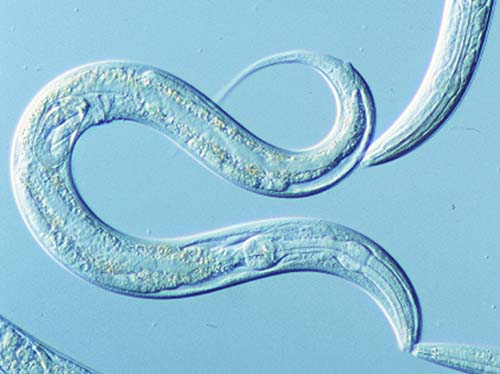
\includegraphics[width=0.35\linewidth]{celegans.jpg}
			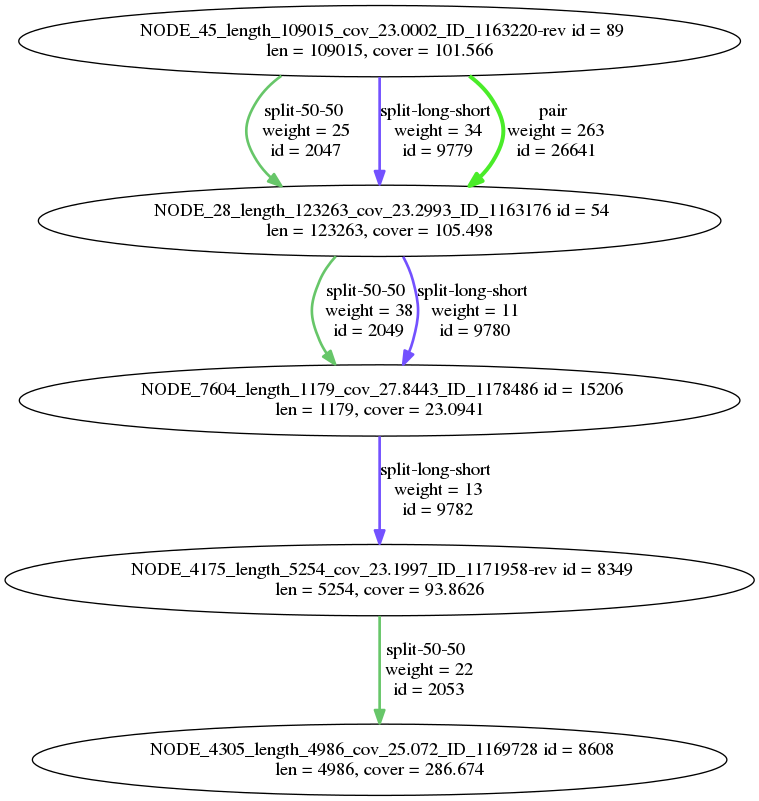
\includegraphics[width=0.35\linewidth]{celegExmp.png}
		\end{center}
	\end{itemize}
\end{frame}

\section{Использованные инструменты}
\begin{frame}[t]{Использованные инструменты}
\begin{itemize}
	\item Язык разработки - \textbf{С++}
	\item \textbf{SeqAn} - библиотека для работы с 
	файлами в SAM/BAM и fasta/fastq форматах.  
	\item \textbf{gtest} - библиотека для тестирования.
	\item Программы для выранивания - \textbf{STAR, nucmer, bowtie2}. 
	\item \textbf{QUAST} - для анализа качетсва сборки. 
	\item \textbf{Tablet} - для визуализации выравненых ридов. 
\end{itemize}
\end{frame}

\section{Дальнейшие пути развития}
\begin{frame}[t]{Дальнейшее развитие}
	\begin{itemize}
		\item Подбор и тестирование 
		приложения на различных 
		данных. Например на данных A.thaliana.
		\cimg{athaliana.jpg}{0.20}
		
		\item Ускорение работы приложения. 
		
		\item Новые способы фильтрации связей и декомпозиции графа. 
		
		\item Нахождение путей в графе и улучшение сборки. 
	\end{itemize}
\end{frame}

\section{Спасибо за внимание}
\begin{frame}{Спасибо за внимание}
    \begin{center}
        Репозиторий: https://github.com/olga24912/bio\_scaffolder
    \end{center}
\end{frame}
\end{document}
